\section{Grundlagen Drehfeldmaschinen}
    \subsection{Dreiphasenwechselstrom (Drehstrom)}
        \begin{minipage}{8cm}
            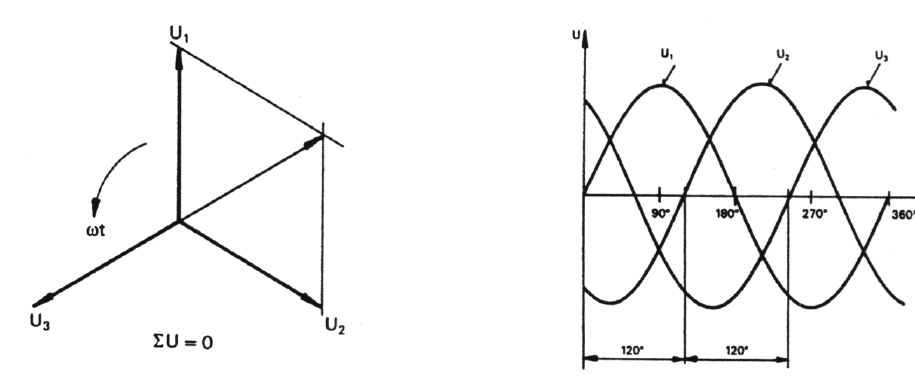
\includegraphics[width=7.5cm]{images/Drehstrom.png}
        \end{minipage}
        \begin{minipage}{10cm}
            Zeiger drehen mit $\omega t$ im Gegenuhrzeigersinn ($\omega > 0$). \\
            $\underline{U}_2$ ist gegenüber $\underline{U}_1$ $120^{\circ}$ nacheilend, $\underline{U}_3$ gegenüber $\underline{U}_1$ $240^{\circ}$.\\
            \\
            Somit gilt (bei symmetrischer Belastung): \\
            $\underline{U}_2 = \underline{U}_1 \cdot e^{j (-120^{\circ})}; \underline{U}_3 = \underline{U}_1 \cdot e^{j (-240^{\circ})} = \underline{U}_1 \cdot e^{j (120^{\circ})}$
        \end{minipage}
    \subsubsection{Stern- (Y) / Dreieckschaltung ($\Delta$)}
        \renewcommand{\arraystretch}{2}
        \begin{tabular}{| p{4.5cm} | l | l |}
            \hline
            &
            Sternschaltung (Y) &
            Dreieckschaltung ($\Delta$) \\
            \hline
            \vspace{0.2cm} &
            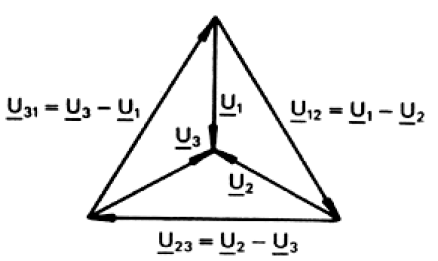
\includegraphics[width=5cm]{images/Sternspannung.png} &
            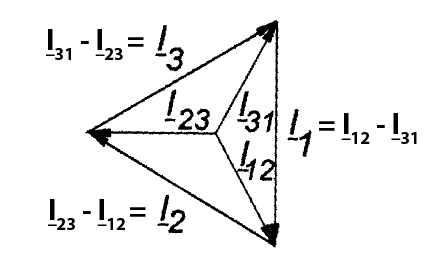
\includegraphics[width=5cm]{images/Dreieckstrom.png} \\
            \hline
            Verkettete Spannung &
            $U = U_{Str} \cdot \sqrt{3}$ \hspace{0.2cm} $\underline{U} = \underline{U}_{Str} \cdot \sqrt{3} \cdot e^{j 30^\circ}$ &
            $U = U_{Str}$ \hspace{0.2cm} $\underline{U} = \underline{U}_{Str}$ \\
            \hline
            Aussenleiterströme &
            $I = I_{Str}$ \hspace{0.2cm} $\underline{I} = \underline{I}_{Str}$ &
            $I = I_{Str} \cdot \sqrt{3} $ \hspace{0.2cm} $\underline{I} = \underline{I}_{Str} \cdot \sqrt{3} \cdot e^{-j 30^\circ} $ \\
            \hline
            Gesamt-Scheinleistung &
            $S = 3 \cdot S_{Str} =\sqrt{3} \cdot U \cdot I $ \hspace{0.2cm} in $[VA]$ &
            $S = 3 \cdot S_{Str} = \sqrt{3} \cdot U \cdot I$ \hspace{0.2cm} in $[VA]$ \\
            \hline
            Scheinleistung pro Strang &
            \multicolumn{2}{l|}{\hspace{3cm} $S_{Str} = U_{Str} \cdot I_{Str}$ \hspace{0.2cm} in $[VA]$} \\
            \hline
            Wirkleistung &
            \multicolumn{2}{l|}{\hspace{3cm} $P = S \cdot \cos\varphi = \sqrt{3} \cdot U \cdot I \cdot \cos\varphi$ \hspace{0.2cm} in $[W]$} \\
            \hline
            Blindleistung &
            \multicolumn{2}{l|}{\hspace{3cm} $Q = S \cdot \sin\varphi = \sqrt{3} \cdot U \cdot I \cdot \sin\varphi$ \hspace{0.2cm} in $[var]$} \\
            \hline
        \end{tabular}
        \renewcommand{\arraystretch}{1.5}

    \subsubsection{Stern-Dreieck-Umwandlung}
        \begin{minipage}[lt]{7.5 cm}
            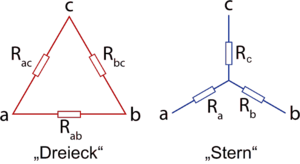
\includegraphics[width=6cm]{images/stern-dreieck.png}
        \end{minipage}
        \begin{minipage}[rt]{9.35 cm} %BASTEL!!
            \renewcommand{\arraystretch}{2}
            \begin{tabular}{ll}
                Umwandlung $\triangle \rightarrow Y$: &
                $Z_{c} = \dfrac{Z_{ac} Z_{bc}}{Z_{ab}+Z_{bc}+Z_{ac}}$ \\
                Umwandlung $Y \rightarrow \triangle$: &
                $Y_{ac}=\dfrac{Y_{a} Y_{c}}{Y_{a}+Y_{b}+Y_{c}}$ \\
                Bei gleichen Widerständen: &
                $R_Y = \frac{R_\triangle}{3}$ \\
                Bei gleichen Kapazitäten: &
                $C_Y = C_\triangle \cdot 3 $ \\
                Bei gleichen Induktivitäten: &
                $L_Y = \frac{L_\triangle}{3}$
            \end{tabular}
            \renewcommand{\arraystretch}{1.5}
        \end{minipage}
        
    \subsection{Feld in einer Drehstrommaschine}
        \begin{minipage}{7cm}
            \abb{images/Drehfeld.png}{6cm}{Entstehung eines Drehfeldes in einem elMaschine}
        \end{minipage}
        \begin{minipage}{11cm}
            Bei einem Drehfeld entsteht zu jedem Zeitpunkt gleichgrosses Magnetisches Feld, woraus dann ein gleichmässiges Drehmoment resultieren kann. Nach dem obrigen Bild dreht sich das Feld in einer Periode um die eigene Achse. Verwendet man mehrere Polpaare wird die Drehzahl reduziert \\
            $Drehfelddrehzahl  = n_d =\frac{f}{p}$ \\
        \end{minipage}

    \subsubsection{Schlupf}
        Als Schlupf bezeichnet man die Beziehung zwischen Drehfelddrehzahl und Läuferdrehzahl. Sie wird mit folgender Formel beschrieben: \\
        \begin{minipage}{8cm}
            $Schlupf = s = \frac{n_d - n}{n_d}$ \\
            Das heisst bei einer Läuferdrehzahl $<$ $n_d$ in Drehfeldrichtung ist der Schlupf 0 $<$ s $<$ 1
        \end{minipage}
        \begin{minipage}{9cm}
            \abb{images/Schlupfgerade.png}{4cm}{Schlupfgerade}
        \end{minipage}
    \newpage